\chapter{QCI和AI-FML}

使用\href{https://kws.oaselab.org/qciai/}{QCI\&AI-FML 學習平台}建立休閒旅遊推薦CI模型。
\section{休閒旅遊推薦模型}
首先要先建立模型規則,模型中有三個輸入變數,分別是花費(Expense)、評估(Evaluation)、距離(Distance)。以及一個輸出推薦程度。每個變數中都分別有三個語意項來區分他們的高低程度。例如,花費變數中的語意項為低(Low)、中(Meduium)、高(High)。 \\

\subsection{輸入輸出變數設定}
使用學習平台設定變數名稱以及它們的單位、邊界值。
\begin{figure}[htbp!]
    \centering
    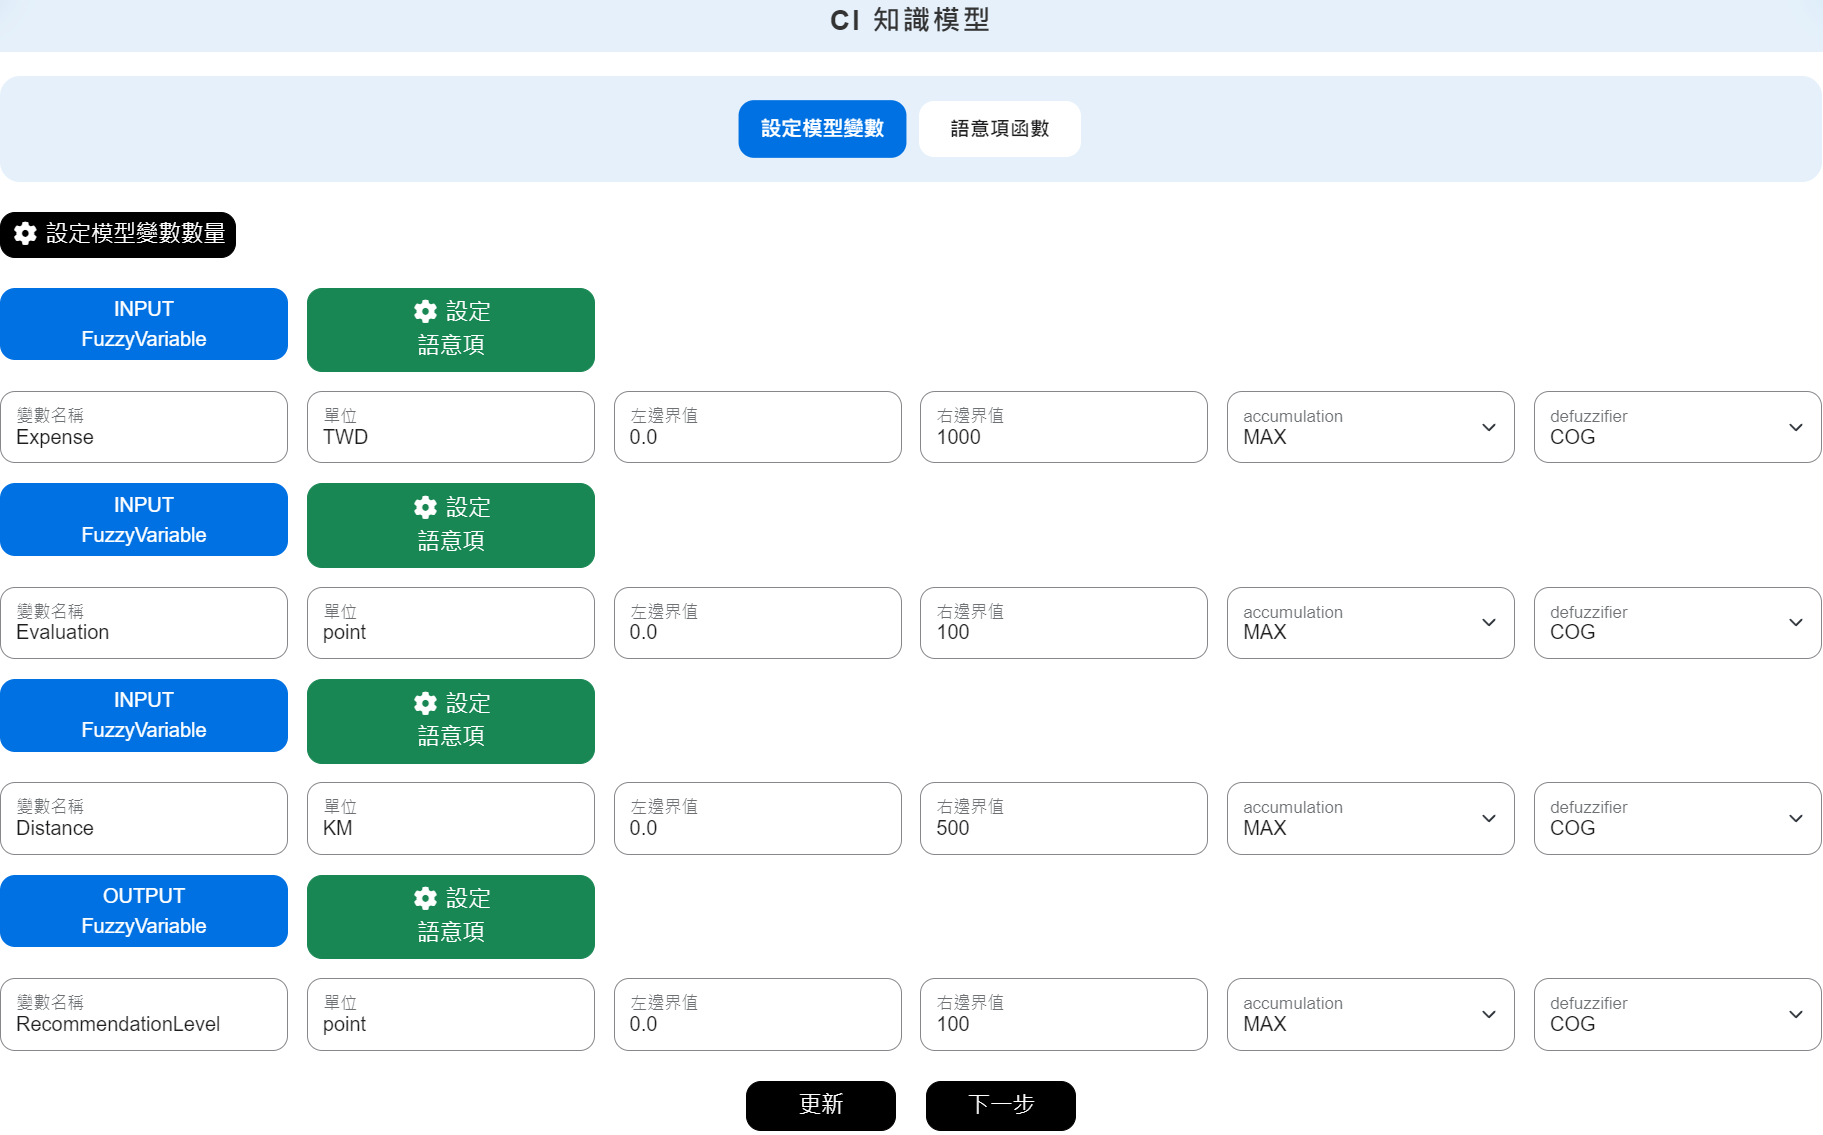
\includegraphics[width=0.6\linewidth]{images/w4/CI_knowledge.png}
    \caption{CI知識模型設定}
    \label{fig:CI-knowledge}
\end{figure}
\newpage

\subsection{語意項設定}
分別設定每個變數中的語意項,\autoref{fig:CI-Expense} 是花費(Expense)的語意項設定及函數圖形。
\begin{figure}[htbp!]
    \centering
    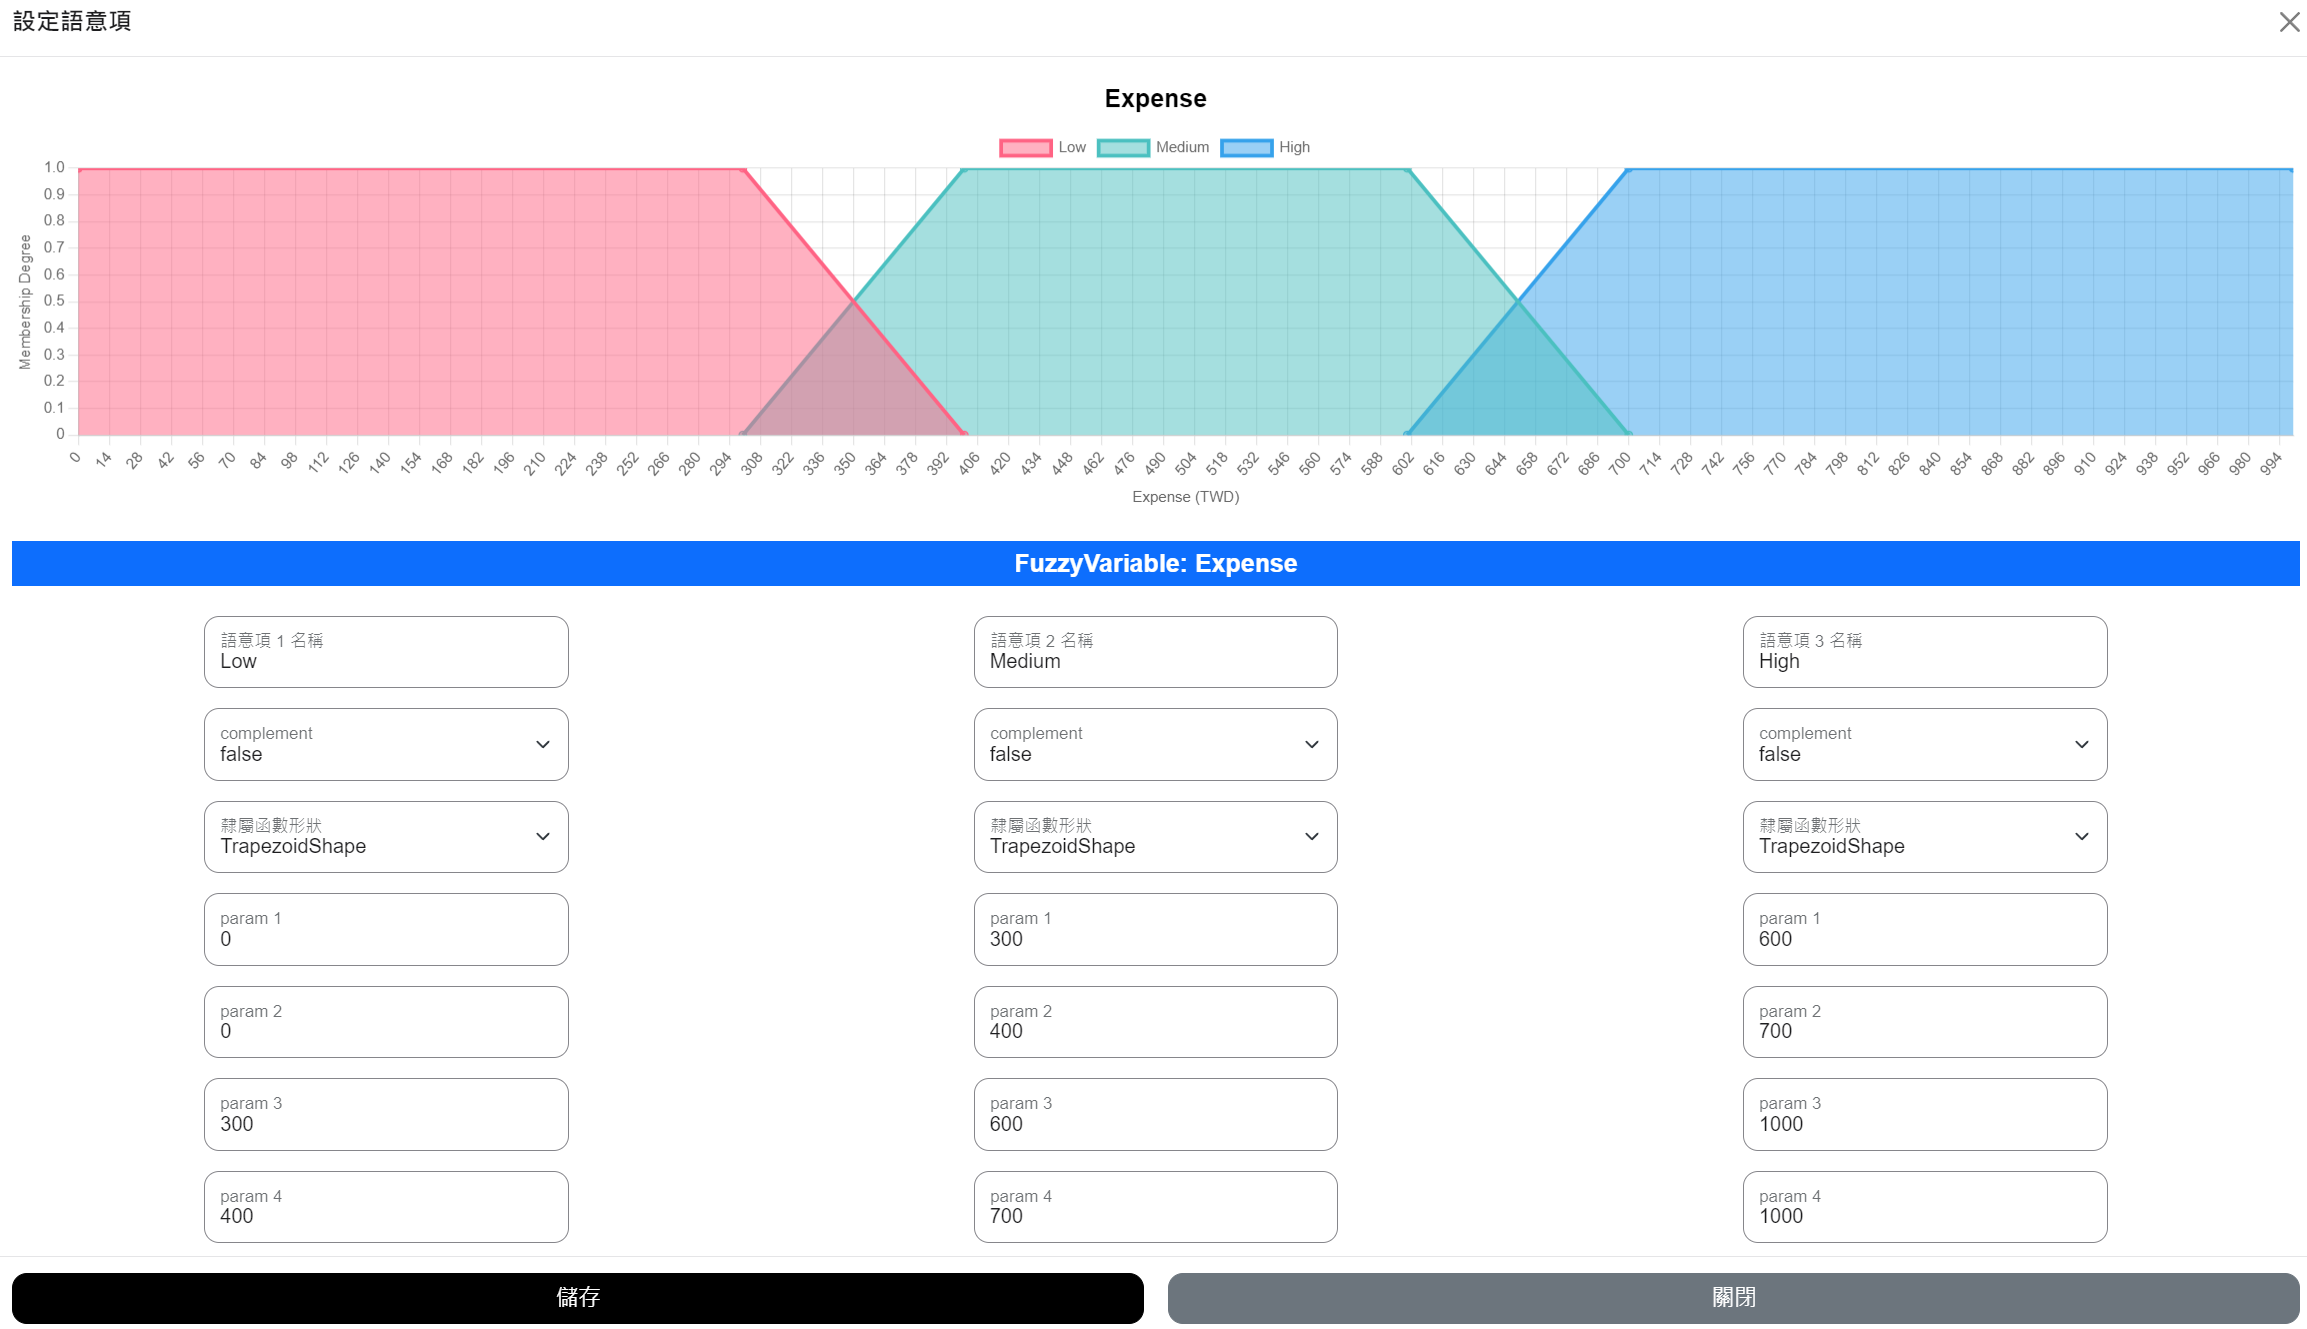
\includegraphics[width=0.5\linewidth]{images/w4/CI_knowledge_setting.png}
    \caption{花費(Expense)語意項設定}
    \label{fig:CI-Expense}
\end{figure}
\begin{figure}[htbp!]
    \centering
    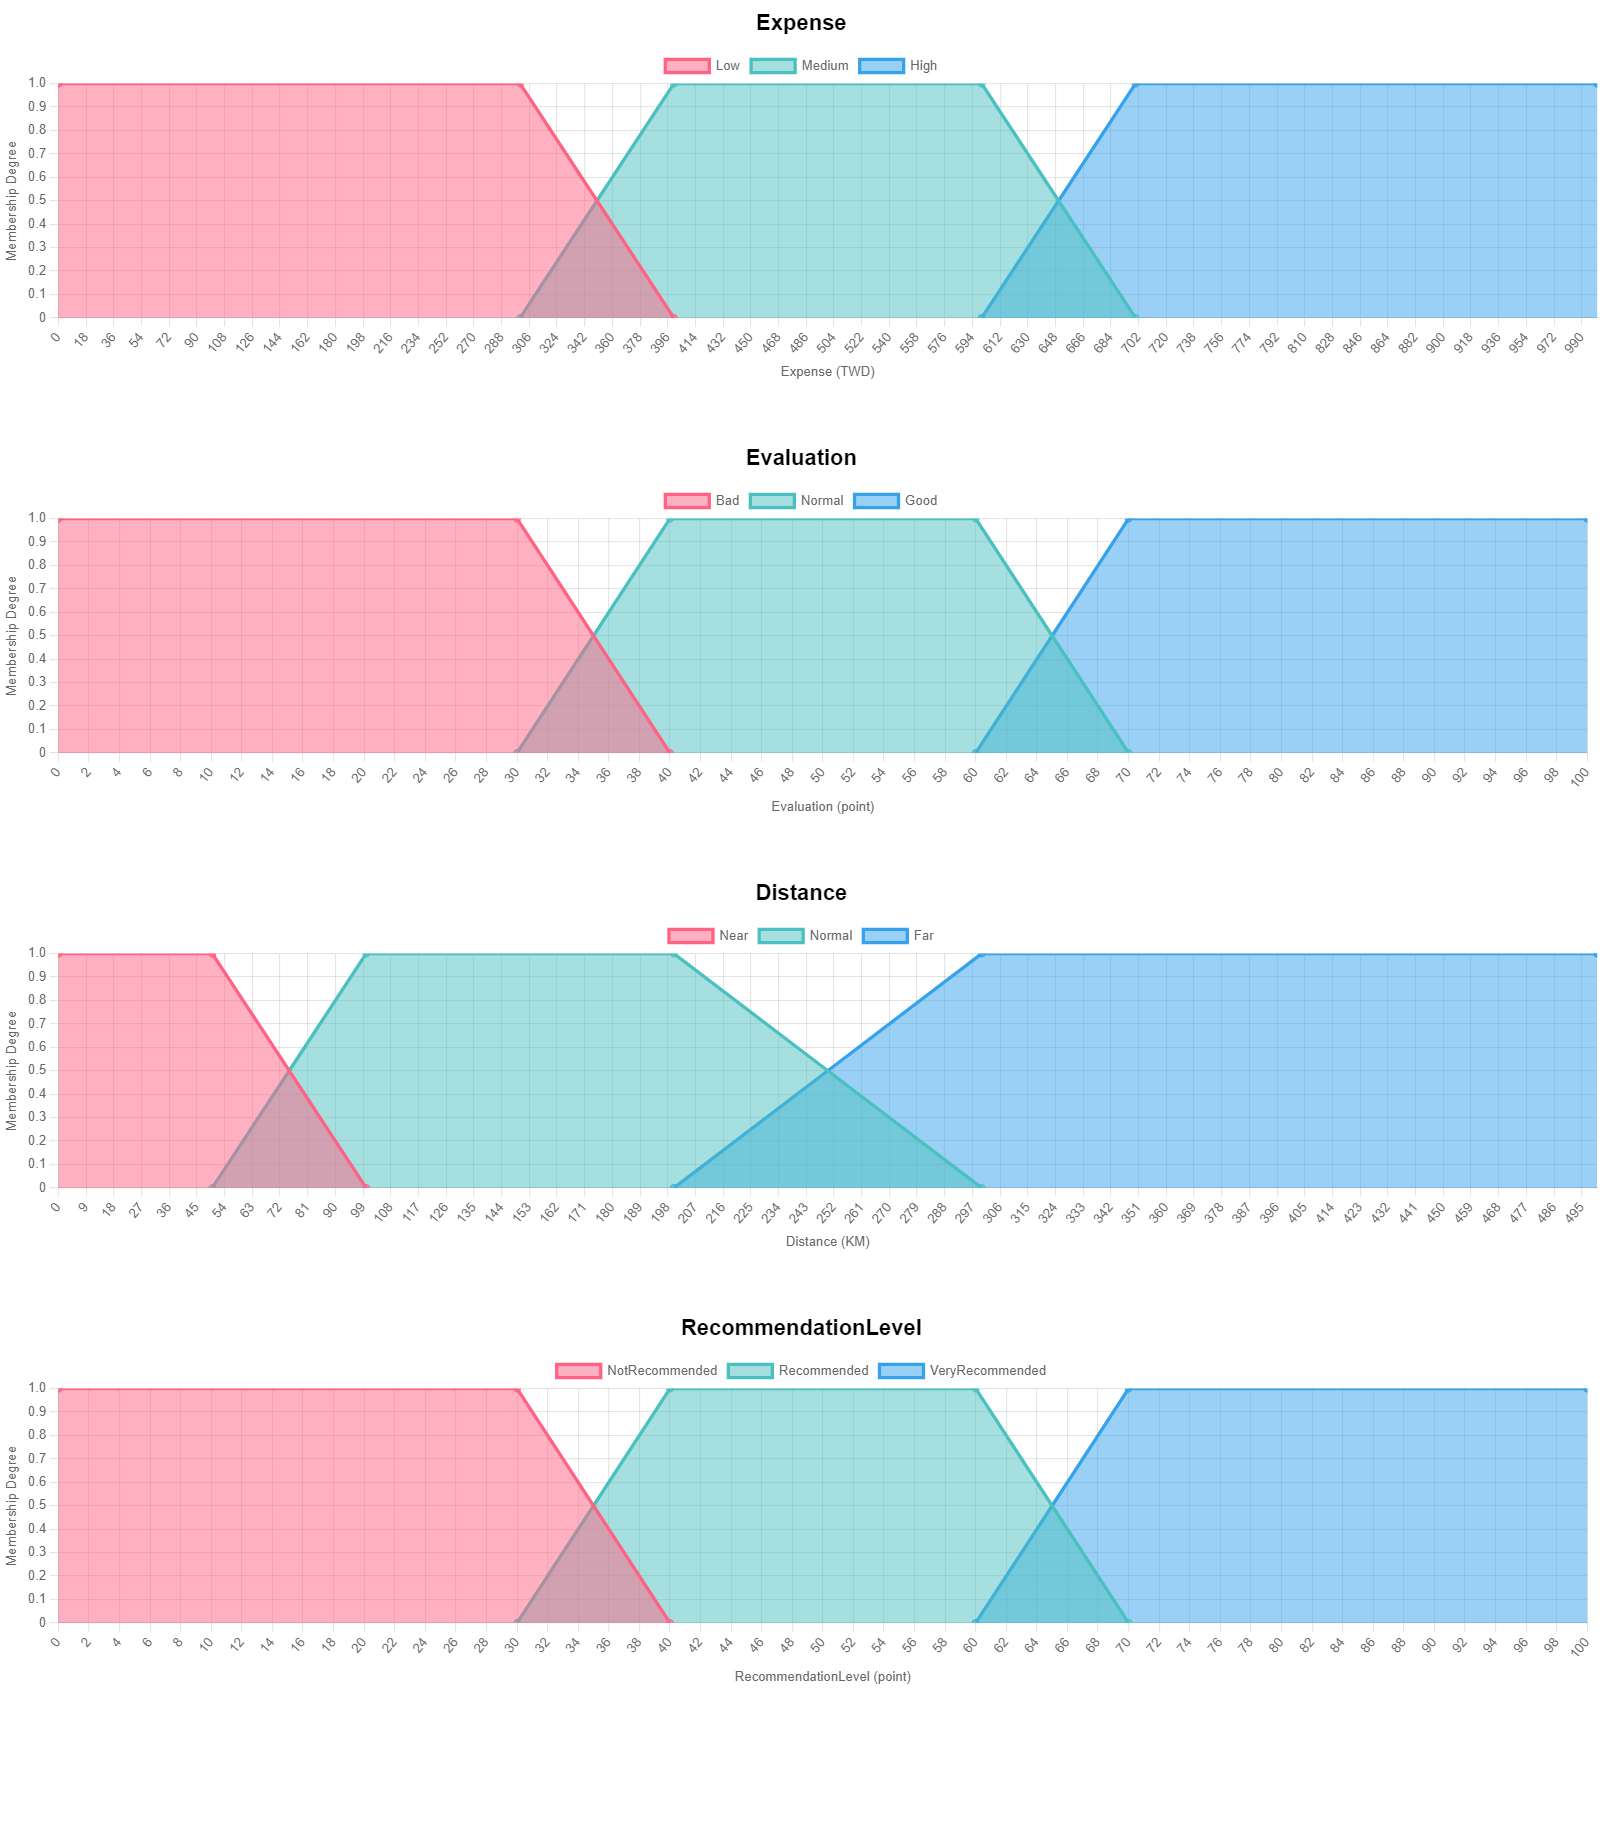
\includegraphics[width=0.5\linewidth]{images/w4/all.png}
    \caption{所有語意項函數圖形}
    \label{fig:all-function}
\end{figure}
\newpage
\subsection{CI推論模型}
因為每個變數有三個語意項,所以總共會有$3^3=27$條規則。根據價錢、距離、評價建立規則庫來評估該次旅遊的推薦等級(\autoref{fig:excel-rule})。
把規則庫導入到學習平台產生推論模型架構(\autoref{fig:inference-model})。
\begin{figure}[htbp!]
    \centering
    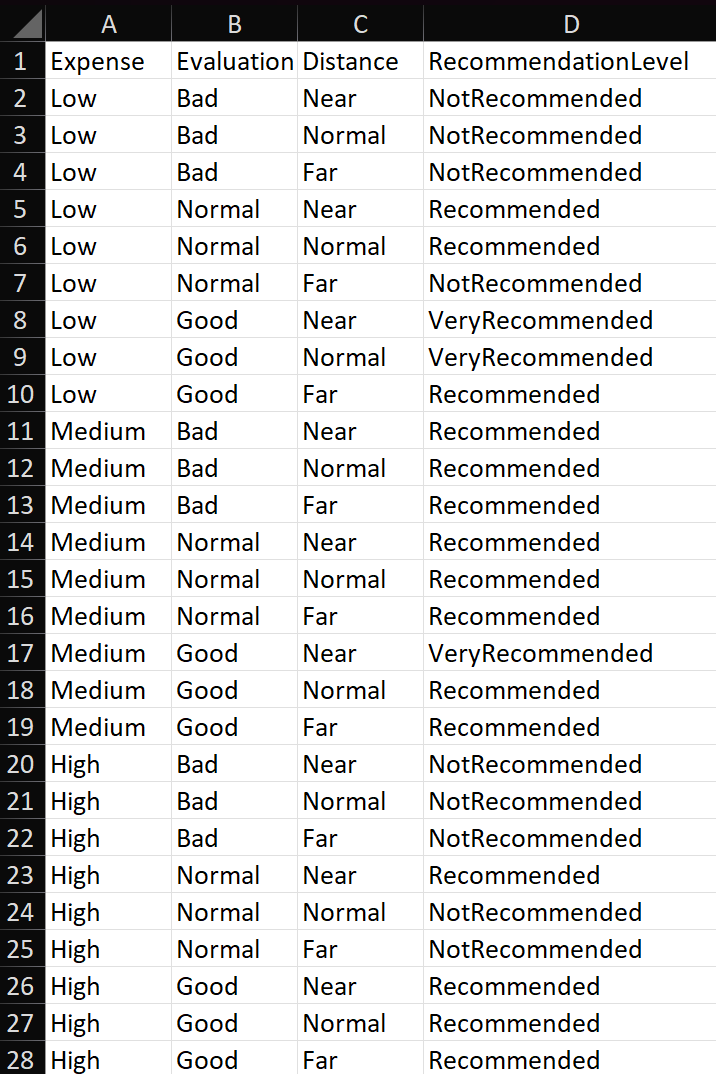
\includegraphics[width=0.45\linewidth]{images/w4/excel-rule.png}
    \caption{旅遊推薦規則}
    \label{fig:excel-rule}
\end{figure}

\begin{figure}[htbp!]
    \centering
    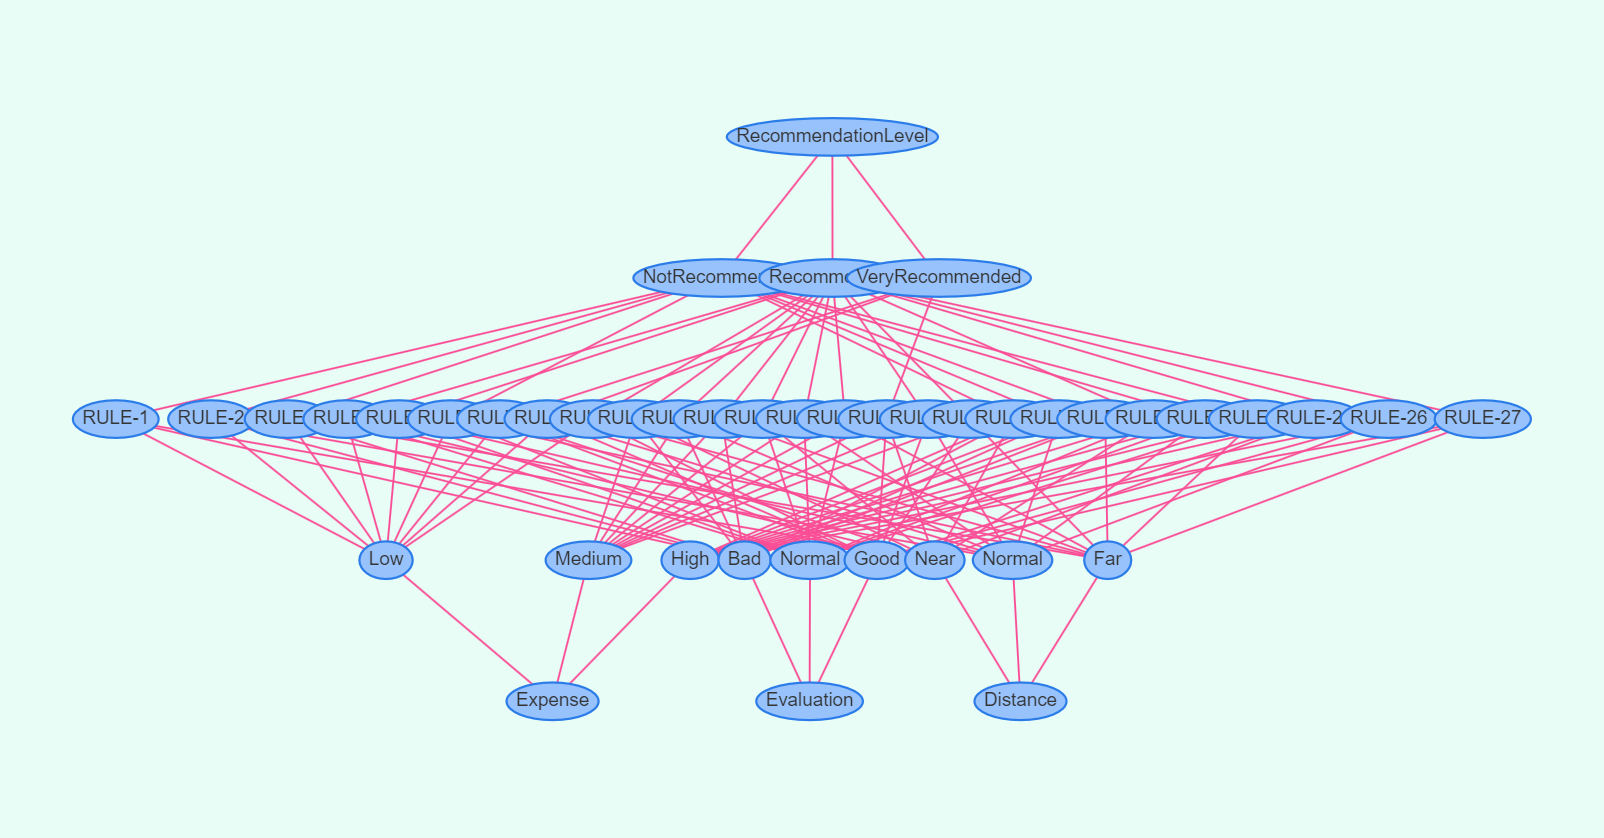
\includegraphics[width=0.8\linewidth]{images/w4/CI-rule.png}
    \caption{推論模型架構}
    \label{fig:inference-model}
\end{figure}

\subsection{串接學習工具}
有了CI模型後串接學習工具,它就會根據傳送的資料顯示推不推薦。
\begin{figure}[htbp!]
    \centering
    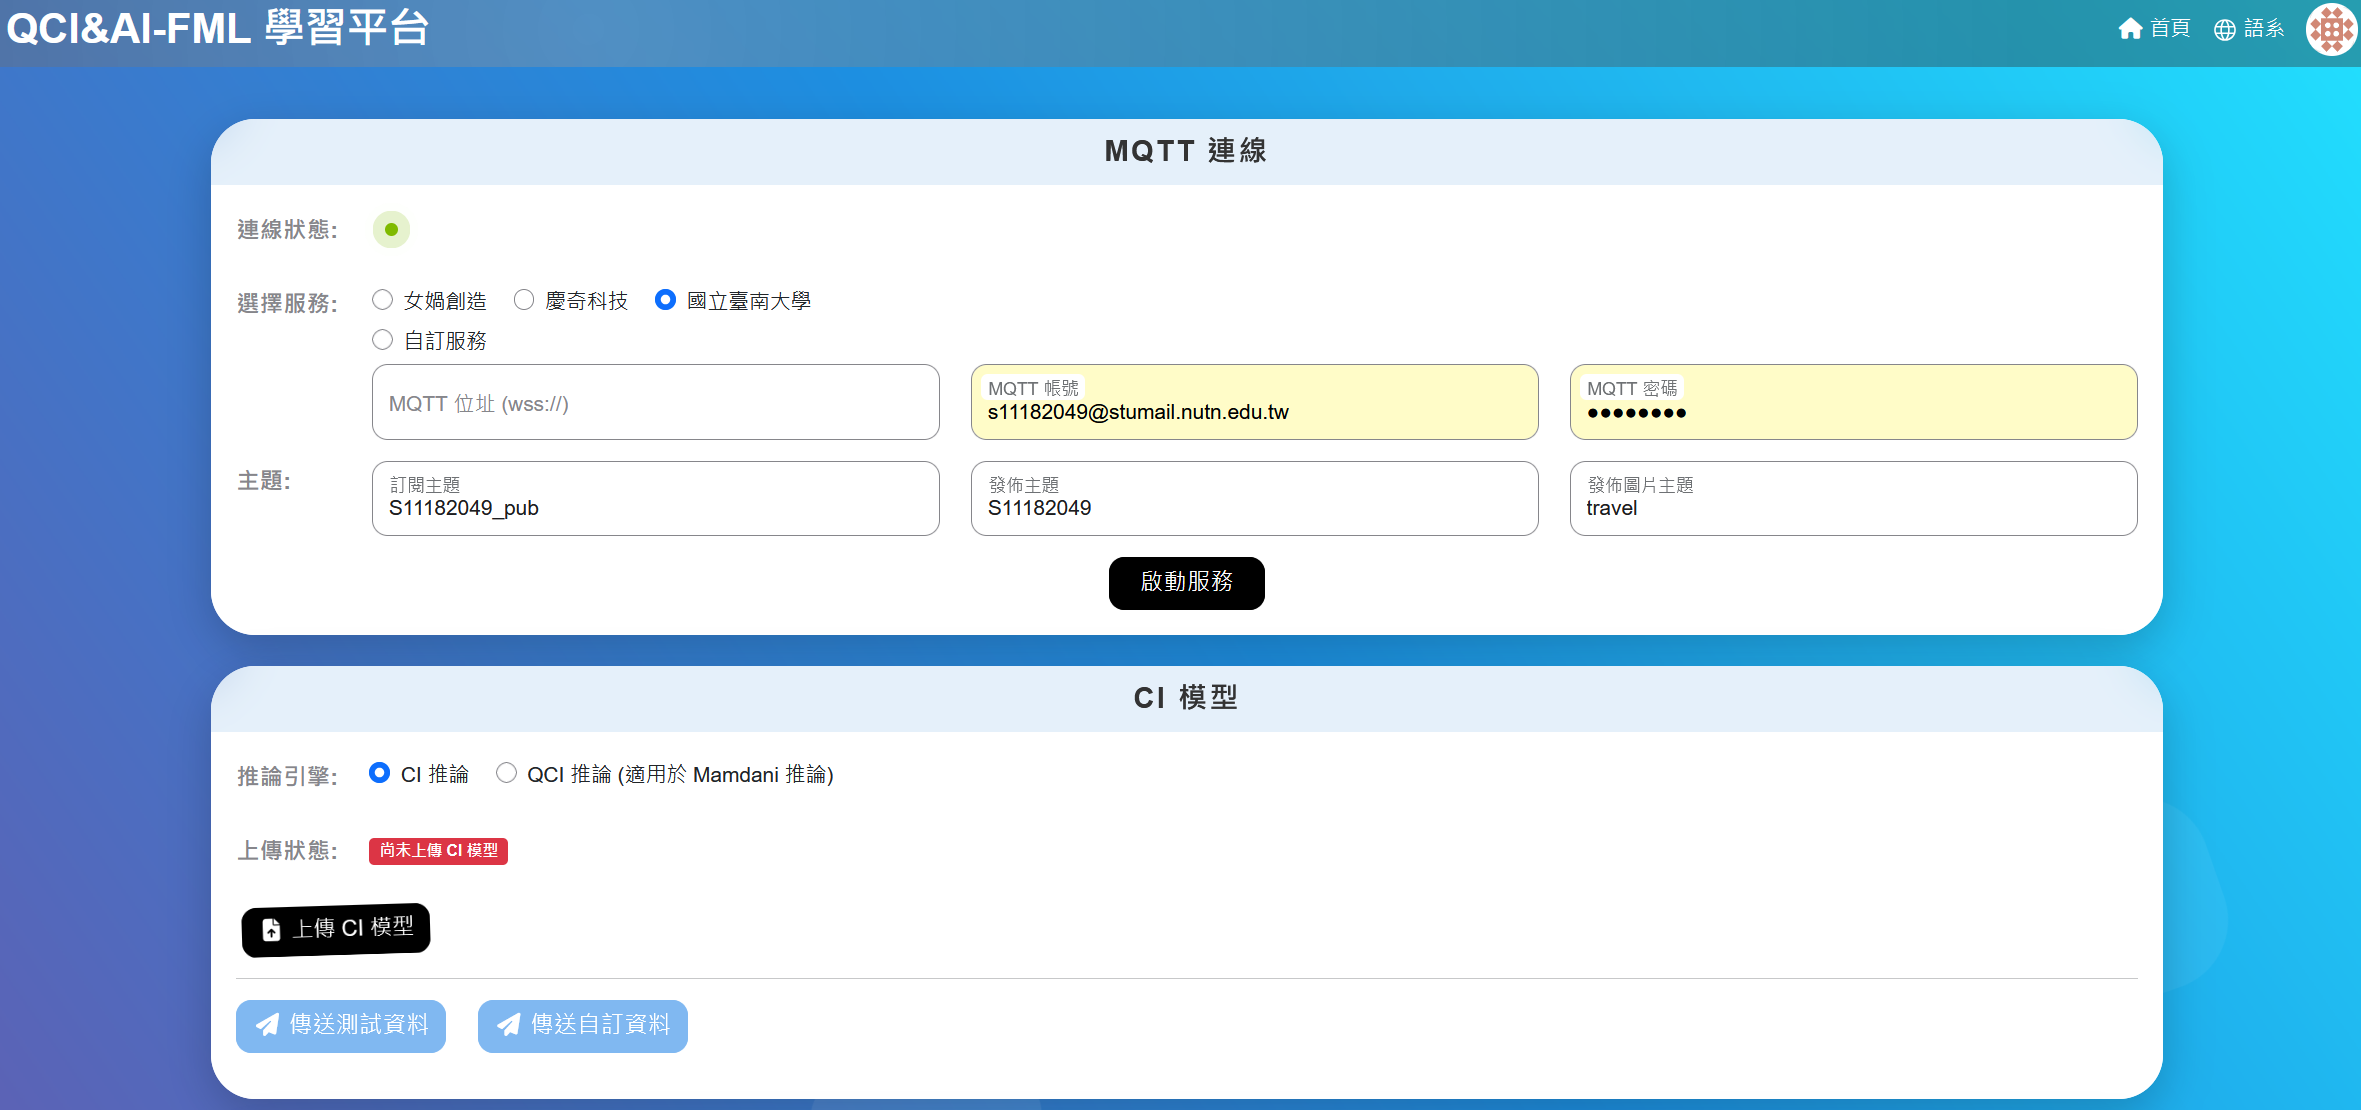
\includegraphics[width=0.7\linewidth]{images/w6/MQTT.png}
    \caption{MQTT連線串接學習工具}
    \label{fig:MQTT}
\end{figure}

\begin{figure}[htbp!]
	\centering
	% 圖片一(左)
	\begin{minipage}{0.4\linewidth}
		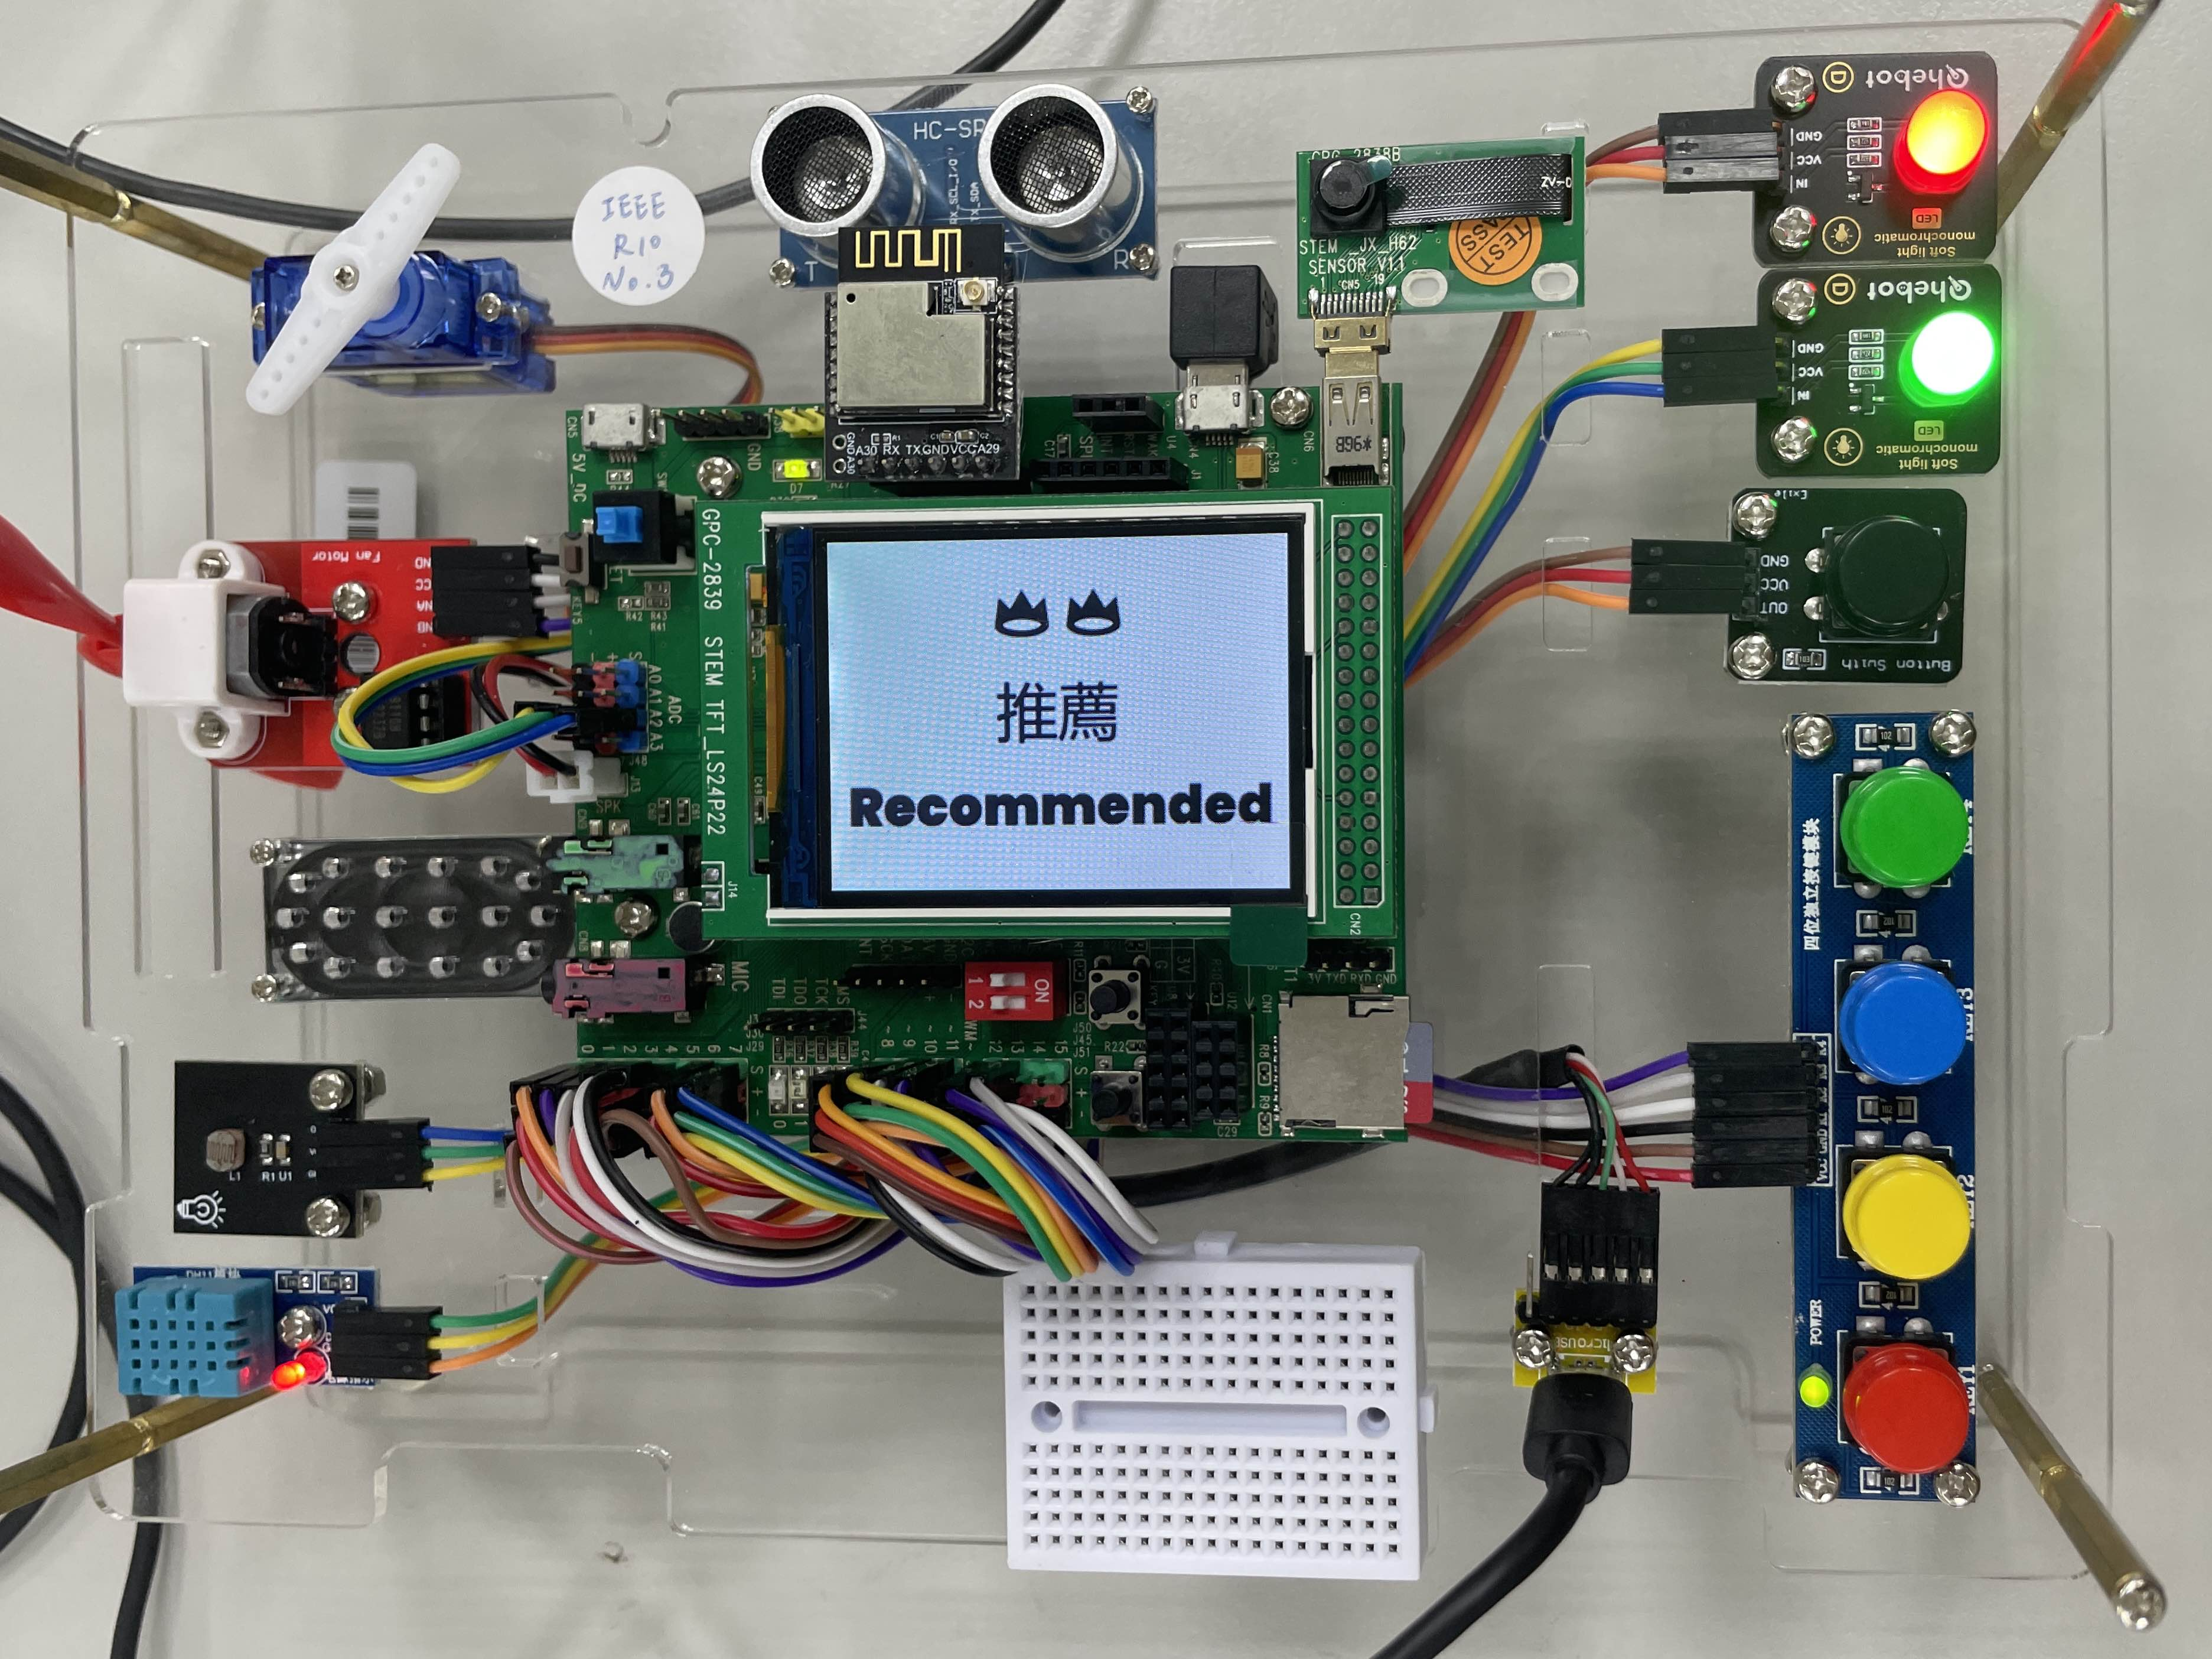
\includegraphics[width=\linewidth]{images/w6/learning-tool-recommend.jpg}
		\caption{學習工具串接-推薦}
	\end{minipage}
	% 圖片二(右)
	\begin{minipage}{0.4\linewidth}
		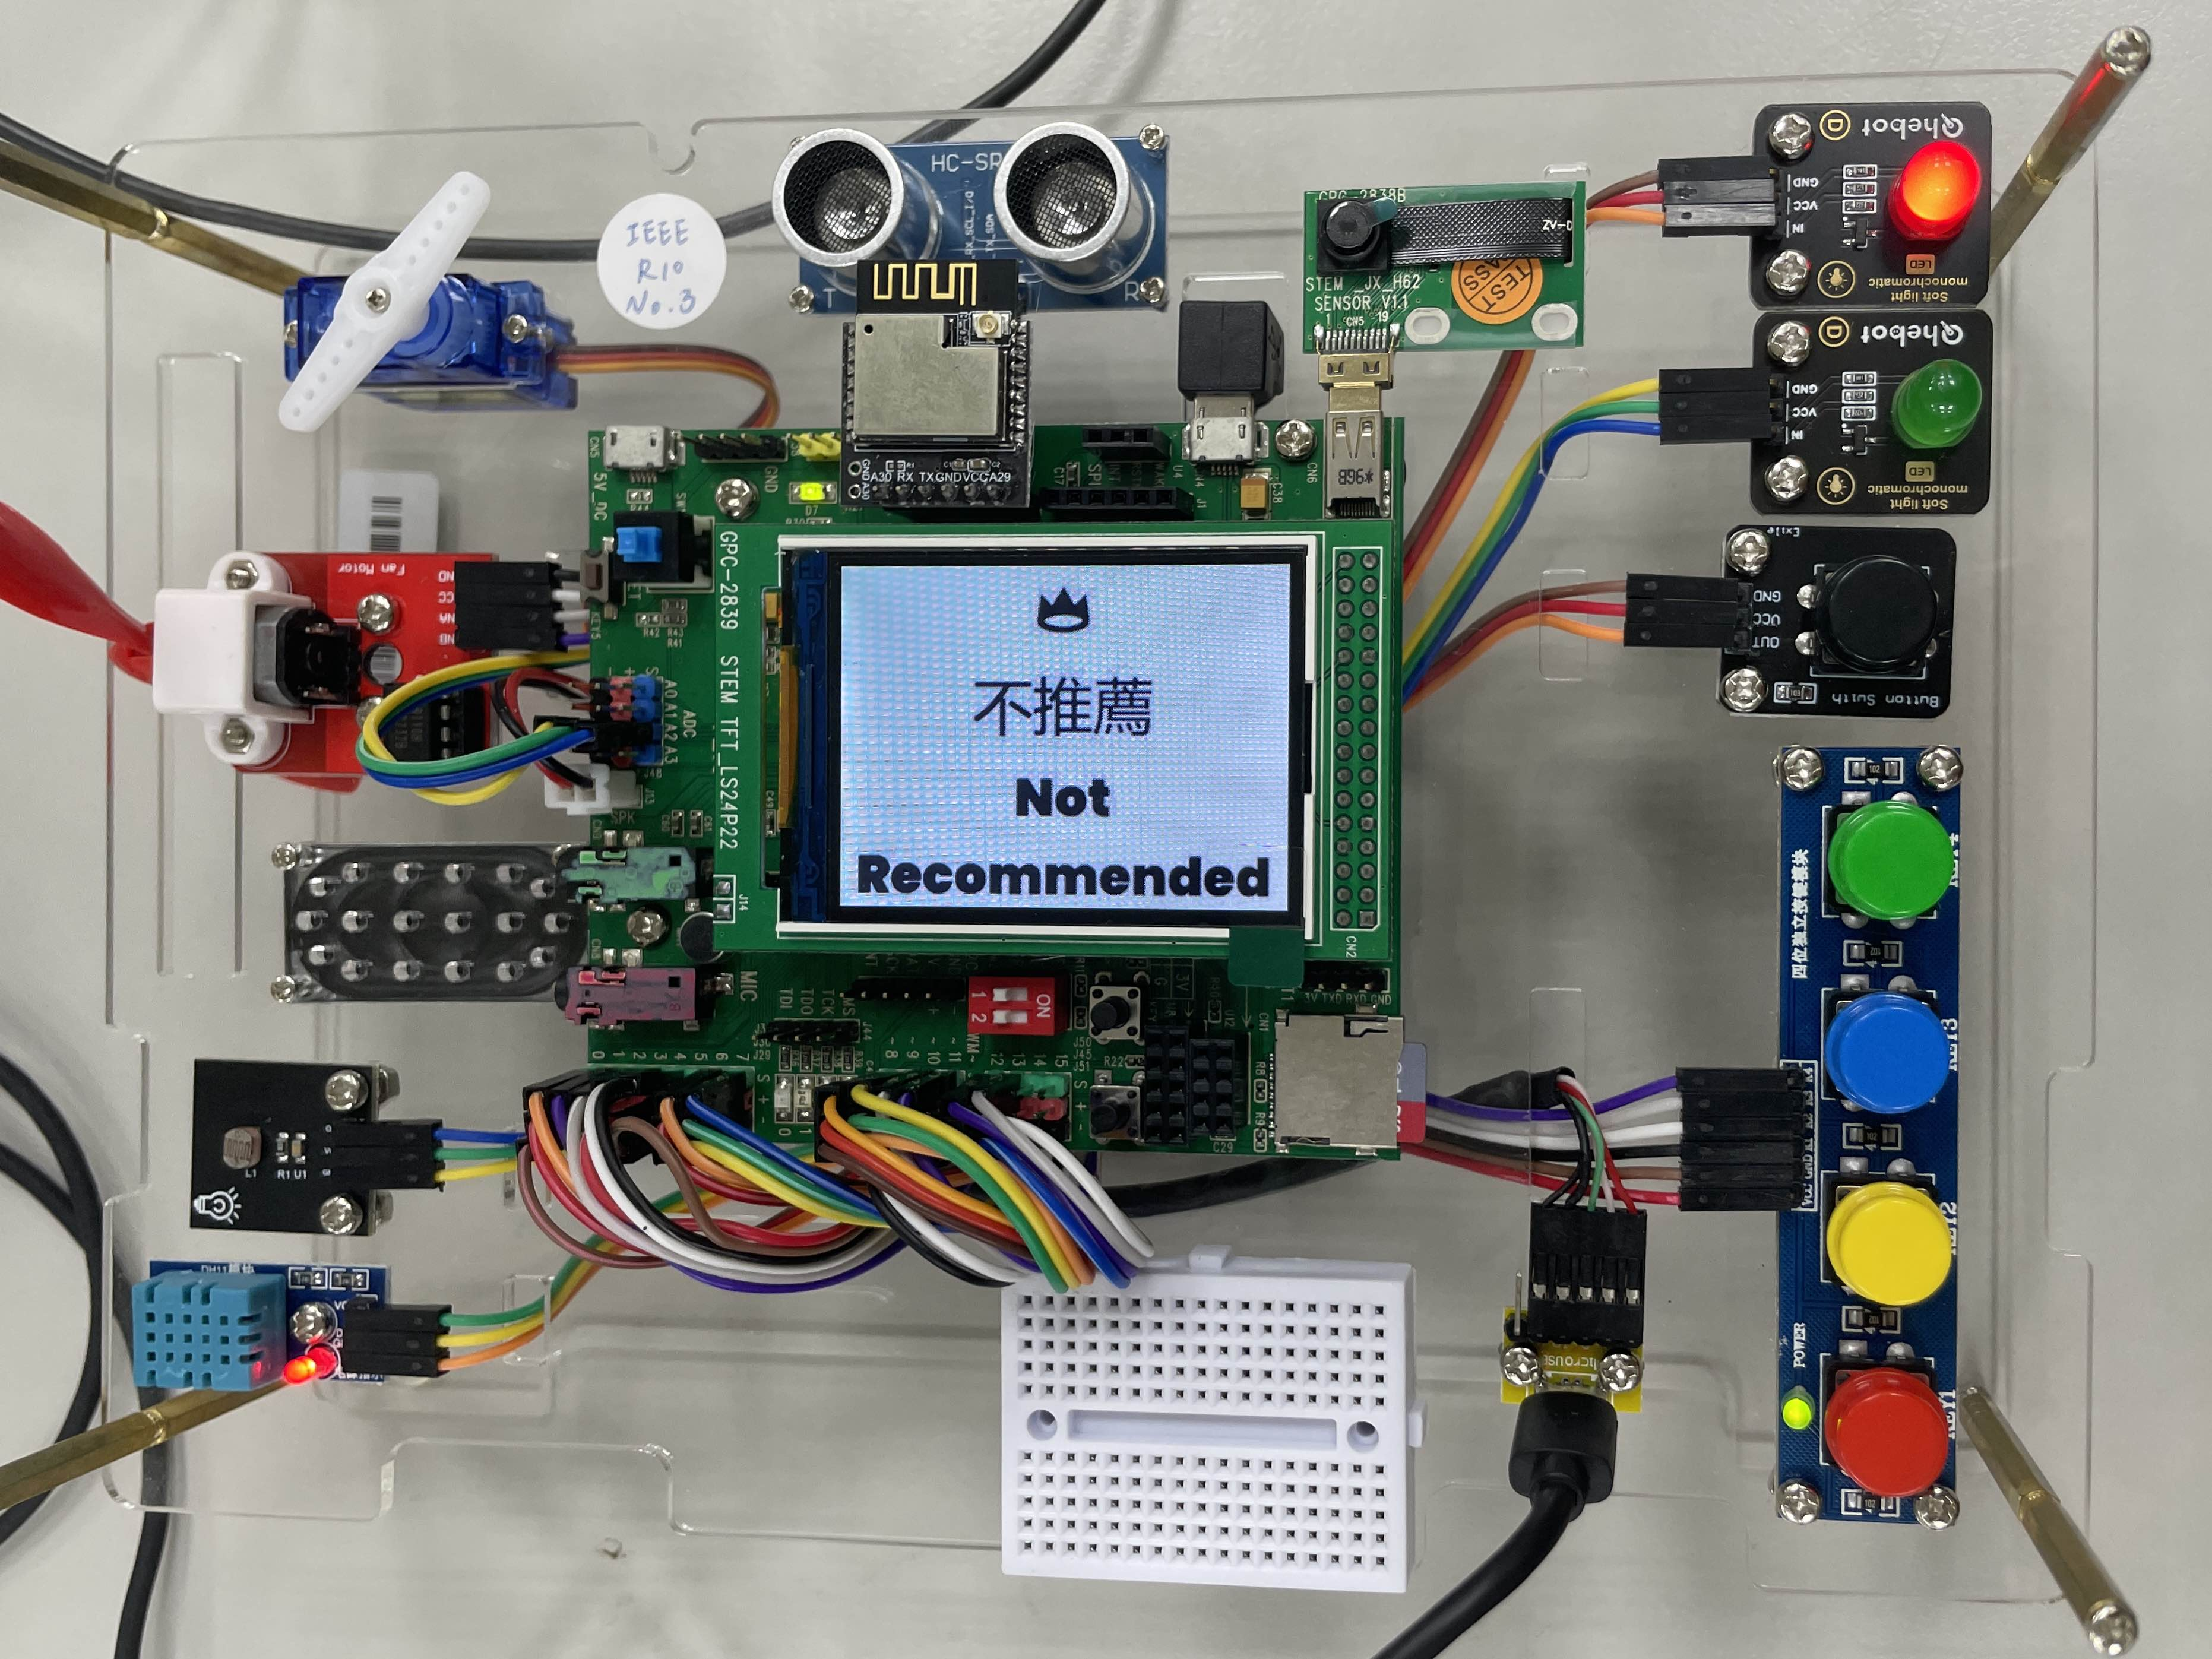
\includegraphics[width=\linewidth]{images/w6/learning-tool-NOTrecommend.jpg}
		\caption{學習工具串接-不推薦}
	\end{minipage}
\end{figure}
